%
% flow design
%

\documentclass[12pt]{article} % FORMAT CHANGE
\usepackage[dvips]{graphicx}
\usepackage{times}

\graphicspath{{./}{figs/}} 

%
% GET THE MARGINS RIGHT, THE UGLY WAY
%
% \topmargin 0.2in
% \textwidth 6.5in
% \textheight 8.75in
% \columnsep 0.25in
% \oddsidemargin 0.0in
% \evensidemargin 0.0in
% \headsep 0.0in
% \headheight 0.0in

\pagestyle{plain}

\addtolength{\hoffset}{-2cm}
\addtolength{\textwidth}{4cm}

\addtolength{\voffset}{-1.5cm}
\addtolength{\textheight}{3cm}

\setlength{\parindent}{0pt}
\setlength{\parskip}{12pt}

\title{Flow Design Document}
\author{PVFS Development Team}
\date{July 2002}

\begin{document}

\maketitle

\section{TODO}
\begin{itemize}
\item point to some other document for explanation of concepts common to all
pvfs2 I/O interfaces (contexts, max idle time, test semantics, etc.)
\end{itemize}

\section{Concepts and Motivation}

Flows are a high level model for how PVFS2 system components
will perform I/O.  It is designed to abstractly but efficiently move
data from source to destination, where source and destination may be
defined as storage devices, network devices, or memory regions.

Features include:

\begin{itemize}

\item \emph{Combining I/O mechanisms}  The flow interface combines
network I/O and disk I/O into a single framework with a scheduler that takes
both into account.

\item \emph{Multiple protocols}
Actual I/O is carried out underneath the flow interface by
\emph{flow protocols}.   We may implement several different
protocols (using different I/O or buffering techniques, for example)
which can be switched at runtime.

\item \emph{Simple interface}  The application interface to
this system will be as high level and simple as possible.  Device
selection, scheduling, buffer management, and request pattern
processing will be transparent to the flow user.  

\item \emph{Datatypes}  Flows allow the user to specify both memory
and file datatypes (similar to those used in MPI) , and will handle
breaking down these datatypes into a format that can be used by lower
level I/O interfaces.

\end{itemize}

\section{Flows}

\subsection{Overview}

A flow describes a movement of data.  The data always moves from a single
source to a single destination.  There may be (and almost always will be)
multiple flows in progress at the same time for different locations-
in particular for clients that are talking simultaneously to several
servers, or servers that are handling simultaneous I/O requests.

At the highest level abstraction, it is important that a flow describes
a movement of data in terms of ``what to do'' rather than ``how to do
it''.  For example, when a user sets up a flow, it may indicate that the
first 100 bytes of a file on a local disk should be sent to
a particular host on the network.  It will not specify what protocols to
use, how to buffer the data, or how to schedule the I/O.  All of this will be
handled underneath the flow interface.  The user just requests that a
high level I/O task be performed and then checks for completion until it
is done.

Note that the ``user'' in the above example is most likely a
system interface or server implementer in pvfs2.  End users will
be unaware of this API.

A single flow created on a server will match exactly one flow on a
client.  For example, if a single client performs a PVFS2 read, the
server will create a storage to network flow, and the client will
create a network to memory flow.  If a client communicates with N servers 
to complete an I/O operation, then it will issue N flows simultaneously.

Flows will not be used for exchanging request protocol messages
between the client and server (requests or acknowledgements).
They will only be used for data transfer.  It is assumed that request
messages will be used for handshaking before or after the flow as 
needed.

\subsection{Architecture}
\label{sec:arch}

There are two major parts of the flow architecture, as seen in figure
\ref{fig:flow-arch}.  The first is the
\emph{flow interface}.  Applications (ie PVFS components) interact with
this interface.  It provides a consistent API regardless of what
protocols are in use, what scheduling is being performed, etc.  

The second major component of the architecture is the \emph{flow
protocol}.
There may be many flow protocols active within one flow interface.  Each
flow protocol implements communication between a different pair of data
endpoint types.  For example, one flow protocol may link TCP/IP to
asynchronous unix I/O, while another may link VIA to memory regions.  For
two seperate hosts to communicate, they must share compatible flow
protocols (as indicated by the dotted line at the bottom of figure
\ref{fig:flow-arch}).

Flow protocols all adhere to a strict interface 
and must provide the same expected functionality (which will be
described later).  Flow protocols take care of details such as buffering
and flow control if necessary.

\begin{figure}
\begin{center}
\caption{Basic flow architecture \label{fig:flow-arch}}
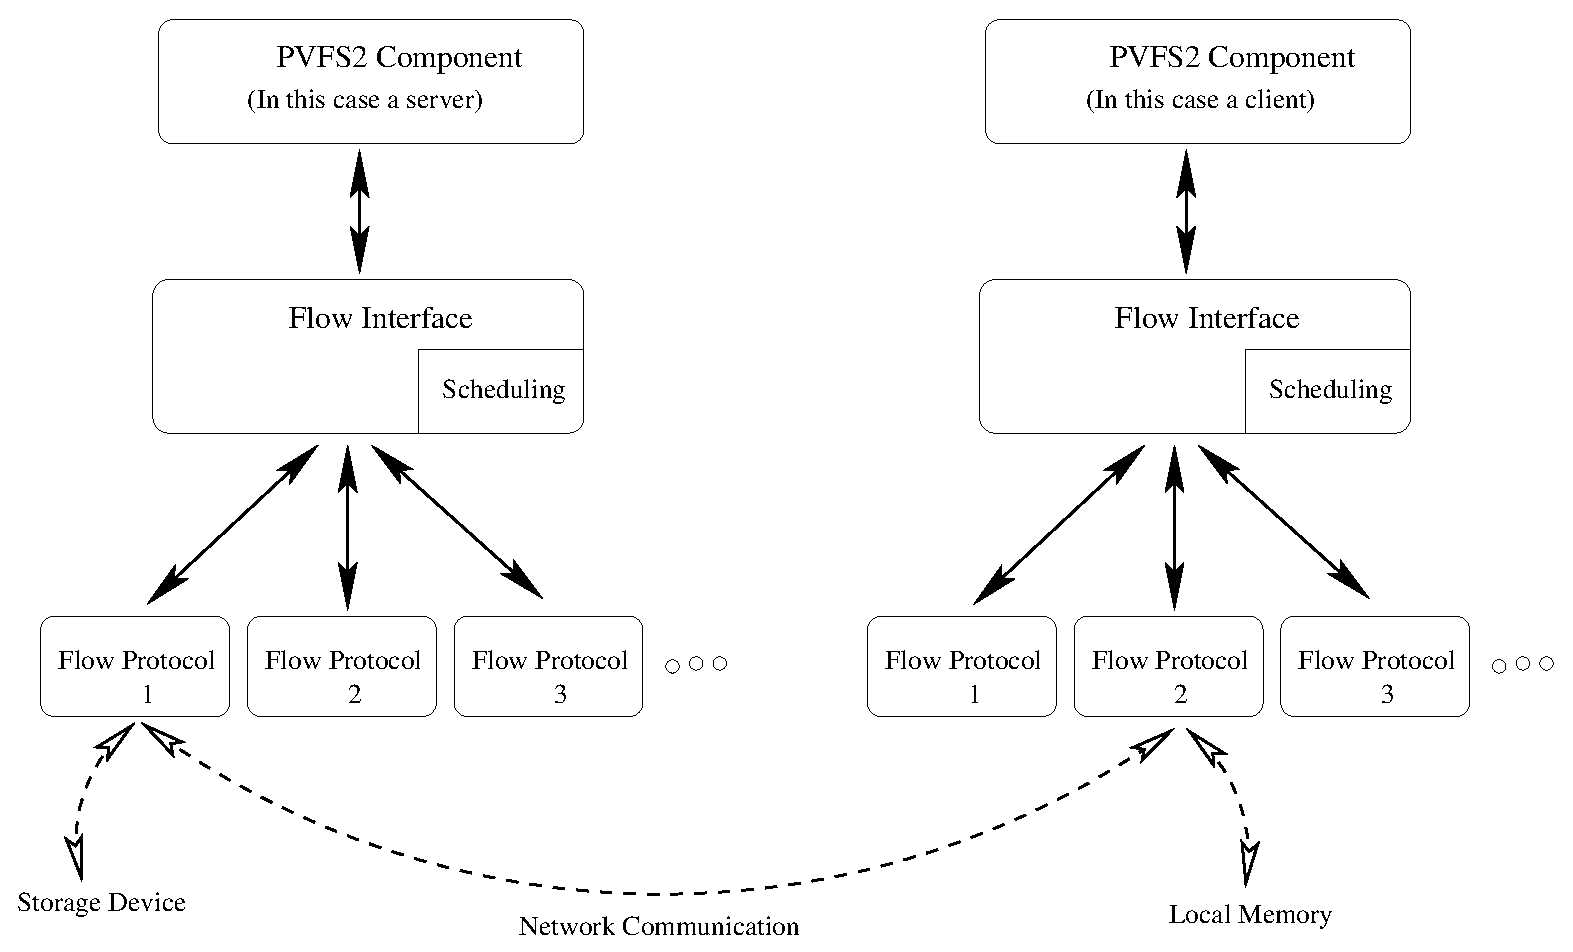
\includegraphics[scale=0.6]{flow-arch.eps}
\end{center}
\end{figure}

\subsection{Describing flows}

Individual flows are represented using structures called \emph{flow
descriptors}.  The source and destination of a given flow are represented
by structures called \emph{endpoints}.  A flow descriptor may serve
many roles.  First of all, when created by a flow interface user, it
describes an I/O task that needs to be performed.  Once it is submitted
to the flow interface, it may keep up with state or progress information.
When the descriptor is finally completed and returned to the user, it will
indicate the status of the completed flow, whether successful or in error.

Flow endpoints describe the memory, storage, or network locations for
the movement of data.   All flow descriptors must have both a 
source and a destination endpoint.

\subsection{Usage assumptions}

It is assumed that all flows in PVFS2 will be \emph{preceded} by a
PVFS2 request protocol exchange between the client and server.  In
a file system read case, the client will send a read request, and
the server will send an acknowledgement (which among other things
indicates how much data is available to be read).  In a file
system write case, the client will send a write request, and the
server will send an acknowledgement that indicates when it is safe
to begin the flow to send data to the server.  Once the flow is completed,
a trailing acknowledgment alerts the client that the server has 
completed the write operation.

The request protocol will transmit information such as file size and 
distribution parameters that may be needed to coordinate remote flows.

\section{Data structures}

\subsection{Flow descriptor}
\label{sec:flow-desc}

Flow descriptors are created by the flow interface user.  At this time,
the caller may edit these fields directly.  Once the flow has been posted
for service, however, the caller may only interact with the descriptor
through functions defined in the flow interface.  It is not safe to
directly edit a flow descriptor while it is in progress.

Once a flow is complete, it is again safe to examine fields within
the descriptor (for example, to determine the status of the
completed flow).

Note that there is an endpoint specific to each type supported by
the flow interface (currently memory, BMI (network), and Trove
(storage)).

The following fields may be set by the caller prior to posting:
\begin{itemize}
\item src: source endpoint (BMI, memory, or Trove addressing information)
\item dest: destination endpoint (BMI, memory, or Trove addressing information)
\item tag: tag used to match up flows with particular operation sequences
\item user\_ptr: void* pointer reserved for use by the caller (may associate a 
flow with some higher level state structure, for example)
\item type: specifies what kind of flow protocol to use for this flow
\item file\_req: file datatype (similar to MPI datatype)
\item file\_req\_offset: offset into the file datatype
\item mem\_req: memory datatype (similar to MPI datatype) (optional)
\item aggregate\_size: total amount of data the flow should transfer (optional)
\item file\_data: struct containing state information about the file to access, used by the distribution subsystem
\end{itemize}

Special notes:  Both the mem\_req and the aggregate\_size fields are optional.
However, at least one of them \emph{must} be set.  Otherwise the flow has 
no way to calculate how much data must be transferred.

The following fields may be read by the caller after completion of a flow:
\begin{itemize}
\item state: final state of flow (see enumerated values in flow.h)
\item error\_code: error code (nonzero if state indicates an error)
\item total\_transfered: amount of data moved by the flow
\end{itemize}

The following fields are reserved for use within the flow code:
\begin{itemize}
\item context\_id: specifies which flow level context the descriptor belongs to
\item flowproto\_id: internal identifier for the flowprotocol used
\item priority: priority level of flow (unused as of yet)
\item sched\_queue\_link: for use by internal scheduler
\item flow\_protocol\_data: void* reserved for flow protocol use
\item file\_req\_state: current state of file datatype processing
\item mem\_req\_state: current state of memory datatype processing
\item result: result of each datatype processing iteration
\end{itemize}

\section{Flow interface}

The flow interface is the set of functions that the flow user is allowed
to interact with.  These functions allow you to do such things as create
flows, post them for service, and check for completion.

\begin{itemize}
	\item \emph{PINT\_flow\_initialize()}: performs initial setup of flow
	interface - must be called once before any other flow interface functions
	\item \emph{PINT\_flow\_finalize()}: shuts down the flow interface
	\item \emph{PINT\_flow\_alloc()}: creates a new flow descriptor
	\item \emph{PINT\_flow\_free()}: frees up a flow descriptor that is
	no longer needed
	\item \emph{PINT\_flow\_reset()}: resets a previously used flow
	descriptor to its initial state and values.
	\item \emph{PINT\_flow\_set\_priority()}: sets the priority of a
	particular flow descriptor.  May be called even when a flow is in
	service.
	\item \emph{PINT\_flow\_get\_priority()}: reads the priority of a
	particular flow descriptor.  May be called even when a flow is in
	service.
	\item \emph{PINT\_flow\_post()}: submits a flow descriptor for
	service
	\item \emph{PINT\_flow\_setinfo()}: used to set optional
	interface parameters.
	\item \emph{PINT\_flow\_getinfo()}: used to read optional
	interface parameters.
\end{itemize}

Three functions are provided to test for completion of posted flows:

\begin{itemize}
	\item \emph{PINT\_flow\_test()}: tests for completion of a single
	flow
	\item \emph{PINT\_flow\_testsome()}: tests for completion of any
   flows from a specified set of flows
	\item \emph{PINT\_flow\_testcontext()}: tests for completion of any
	flows that are in service in the interface 
\end{itemize}

\section{Flow protocol interface}

The flow protocols are modular components capable of moving data between
particular types of endpoints.  (See section \ref{sec:arch} for an
overview).  Any flow protocol implementation must conform to a
predefined flow protocol interface in order to interoperate with the
flow system.  

\begin{itemize}
	\item \emph{flowproto\_initialize()}: Initializes the flow
	protocol (called exactly once before posting any flows)
	\item \emph{flowproto\_finalize()}: shuts down the flow
	protocol (forceful terminating any pending flows)
	\item \emph{flowproto\_post()}: posts a flow descriptor
	\item \emph{flowproto\_find\_serviceable()}: returns an array of active
	flows from the flow protocol that are either completed or in need of
	service
	\item \emph{flowproto\_service()}: performs work on a single
	flow descriptor that is ready for service (as indicated by a
	flowproto\_find\_serviceable() function)
	\item \emph{flowproto\_getinfo()}: reads optional parameters
	from the protocol
	\item \emph{flowproto\_setinfo()}: sets optional protocol
	parameters
\end{itemize}

The following section describing the interaction between the flow component
and the flow protocols may be helpful in clarifying how the above functions
will be used.

\section{Interaction between flow component and flow protocols}

The flow code that resides above the flow protocols serves two primary
functions: multiplexing between the various flow protocols, and scheduling
work.

The multiplexing is handled by simply tracking all active flow protocols and
directing flow descriptors to the appropriate one. 

The scheduling functionality is the more complicated of the two
responsibilities of the flow code.  This responsibility leads to the 
design of the flow protocol interface and the states of the flow descriptors.
In order to understand these states, it is important to understand that 
flow protocols typically operate with a certain granularity that is 
defined by the flow protocol implementation.  For example, a flow protocol 
may transfer data 128 KB of data at a time.  A simple implementation of a memory to 
network flow may post a network send of 128 KB, wait for it to complete, then
post the next send of 128 KB, and so on.  Each of these iterations is driven by
the top level flow component.  In other words, the flow protocol is not 
autonomous.  Rather than work continuously once it receives a flow descriptor, 
it only performs one iteration of work at a time, and then waits for the 
flow component to tell it to continue.  This provides the flow interface
with an opportunity to schedule flows and choose which ones to service at 
each iteration.

When a flow descriptor is waiting for the flow component to allow it to
continue, then it is ``ready for service''.  The flow component may
then call the flowproto\_service() function to allow it to continue.  In 
the above example, this would cause the flow protocol to post another network
send.  

In order to discover which flow descriptors are ``ready for service'' (and 
therefore must be scheduled), it calls flowproto\_find\_serviceable() for each
active flow protocol.  Thus, the service loop of the flow component looks something like this:

\begin{enumerate}
\item call flowproto\_find\_serviceable() for each active flow protocol to
generate a list of flows to service
\item run scheduling algorithm to build list of scheduled flows
\item call flowproto\_service() for each scheduled flow (in order)
\item if a flow descriptor reaches the completed or error state (at any time),
then move it to a list of completed flow descriptors to be returned to the 
caller
\end{enumerate}

The scheduling filter (at the time of this writing) does nothing but service
all flows in order.  More advanced schedulers will be added later.

\subsection{Example flow protocol (implementation)}

The default flow protocol is called "flowproto\_bmi\_trove'' and is capable of
handling the following endpoint combinations:

\begin{itemize}
\item BMI to memory 
\item memory to BMI
\item BMI to Trove
\item Trove to BMI
\end{itemize}

The following summarizes what the principle flow protocol interface functions
do in this protocol:

\begin{itemize}
\item flowproto\_post(): allocates any intermediate buffers that may be needed,
begins datatype processing
\item flowproto\_service(): posts the next necessary BMI and Trove operations
\item flowproto\_find\_serviceable(): tests for completion of pending BMI and 
trove operations, drives the state of any flow descriptors affected by completion, and returns flow descriptors ready for service to caller
\end{itemize}

The flow protocol performs double buffering to keep both the Trove and BMI interfaces as busy as possible when transferring between the two.

The flow protocol does not have an internal thread.  However, if it detects that the job interface is using threads (through the \_\_PVFS2\_JOB\_THREADED\_\_ define), then it will use the job interface's thread manager to push on BMI and 
Trove operations.  The find\_serviceable() function then just checks for
completion notifications from the thread callback functions, rather than
testing the BMI or Trove interfaces directly.

Trove support is compiled out if the \_\_PVFS2\_TROVE\_SUPPORT\_\_ define is
not detected.  This is mainly done in client libraries which do not 
need to use Trove in order to reduce library dependencies.

\section{Implementation note: avoiding flows}

The flow interface will introduce overhead for small operations
that would not otherwise be present.  It may therefore be helpful
to eventually introduce an optimization to avoid the use of flows
for small read or write operations.

\begin{verbatim}

text of an email discussion on this topic (> part by Phil, non >
part by Rob):

> Yeah, we need to get these ideas documented somewhere.  There may actually
> be a couple of eager modes.  By default, BMI only allows unexpected
> messages < 16K or so.  That places a cap on the eager write size,
> unless we had a second eager mode that consists of a) send write request
> b) send write data c) receive ack...

Yes.  These two modes are usually differentiated by the terms "short" and
"eager", where the "short" one puts the data actually into the same
packet/message (depending on the network layer at which we are working).

> Of course all of this would need to be tunable so that we can see what
> works well.  Maybe rules like:
> 
> contig writes < 15K : simple eager write
> 15K < contig writes < 64K : two part eager write
> writes > 64K && noncontig writes : flow
> 
> contig reads < 64K : eager read
> contig reads > 64K && noncontig reads : flow

Yeah, something like that.

\end{verbatim}

\end{document}







